\documentclass[a4paper]{scrartcl}
\usepackage{scrpage2}
\usepackage[ngerman]{babel}
\usepackage[T1]{fontenc}
\usepackage[utf8]{inputenc}
%\usepackage[pdftex]{graphicx}
%\usepackage[intlimits]{amsmath}
%\usepackage{listings}
%\lstset{frame=single,breaklines=true}
\usepackage{ amssymb }
\usepackage{amsmath}
\usepackage{hyperref}
\usepackage{enumerate}
\usepackage[a4paper, total={19cm, 23cm}]{geometry}
\usepackage{stmaryrd}
\usepackage{graphicx}
\pagestyle{scrheadings}
\pagenumbering{gobble}
\ihead{Übungsblatt 4\\Nils Werner 108012219293}
\chead{\\Paul Rösler 108012225686	}
\ohead{Übungsgruppe: Mo. 16:00\\Daniel Teuchert 108012214552}
\setheadsepline{0.4pt}
\begin{document}

\section*{Aufgabe 1}

\newpage
\section*{Aufgabe 2}
\begin{enumerate}[a)]
\item ~\\
\begin{figure}[htp] \centering{
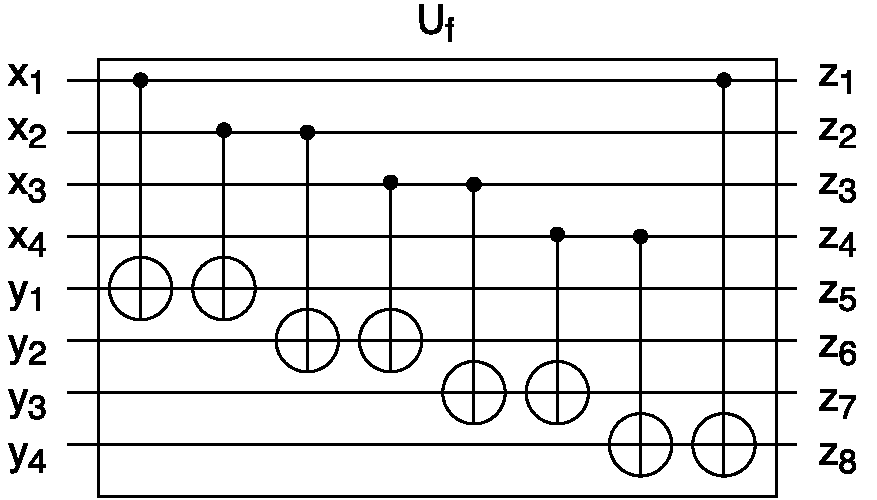
\includegraphics[scale=0.5]{ue4a2a.pdf}}
\caption{Quantenschaltkreis für die reversible Einbettung von $f$}
\end{figure}

\item ~\\
\begin{figure}[htp] \centering{
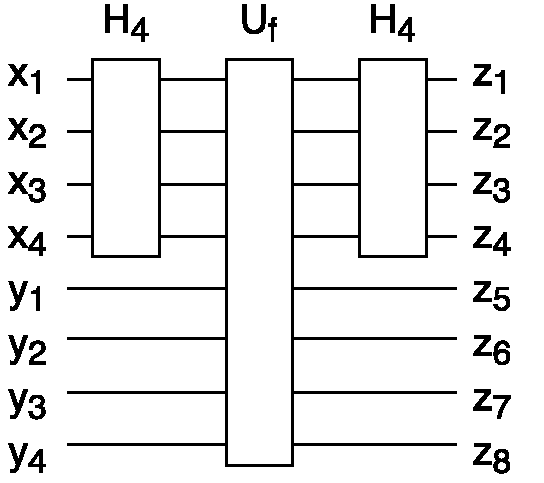
\includegraphics[scale=0.5]{ue4a2b.pdf}}
\caption{Quantenschaltkreis $Q_S$ des Algorithmus von Simon für dieses $f$}
\end{figure}

\item

$ \begin{pmatrix}
1 & 1 & 0 & 0 \\
1 & 0 & 1 & 0 \\
1 & 0 & 0 & 1 \\
0 & 0 & 0 & 0 \\
\end{pmatrix} \begin{pmatrix}
s_1 \\
s_2 \\
s_3 \\
s_4 \\
\end{pmatrix} = \begin{pmatrix}
0 \\
0 \\
0 \\
0 \\
\end{pmatrix} \Leftrightarrow \begin{pmatrix}
s_1 \\
s_1 \\
s_1 \\
0 \\
\end{pmatrix} = \begin{pmatrix}
s_2 \\
s_3 \\
s_4 \\
0 \\
\end{pmatrix}$ \\
$\Rightarrow (s_1, s_2, s_3, s_4) = (1, 1, 1, 1) \vee (s_1, s_2, s_3, s_4) = (0, 0, 0, 0)$
\end{enumerate}

\newpage
\section*{Aufgabe 3}

\newpage
\section*{Aufgabe 4}
\begin{enumerate}[a)]
\item

\item

\item

\item

\item

\item
Algorithmus:\\
\begin{enumerate}[1.]
\item Wähle $a\in_R \mathbb{Z}_N^*$ uniform
\item Berechne \texttt{PERIODE}($N,a$) und erhalte so $t =$ ord$_{\mathbb{Z}_N^*}(a)$ mit $t=2^s\cdot u$
\item Berechne $\frac{a^t}{a^2}+1=x$
\item Berechne ggT($N, x$)$=p$
\item Falls gilt: $p | N$ gebe $p$ aus, sonst gehe zu Schritt 1
\end{enumerate}

Korrektheit:
$x=\frac{a^t}{a}+1= \frac{a^{2^s\cdot u}}{a^2}+1= a^{2^{s-1}\cdot u}+1$\\
Es filt mit Ws $\geq \frac{1}{4}$ dass ggT($N, x$)$=p$ ein nicht-trivialer Teiler von $N$ ist und das somit gilt $p|N$

Laufzeit:



\end{enumerate}


\end{document}
